% Search for all the places that say "PUT SOMETHING HERE".

\documentclass[11pt]{article}
\usepackage{amsmath,textcomp,amssymb,graphicx,enumerate,hyperref,enumitem,mathtools,tikz-qtree,listings,chemformula,bm,graphicx,grffile,gensymb,physics,amssymb,datetime,siunitx}
\graphicspath{{/Users/jonathansun5/Documents/Fall 2017/MCB 166/Homeworks/HW 4/Screen Shot 2017-10-29 at 5.24.09 PM.png} {/Users/jonathansun5/Documents/Fall 2017/MCB 166/Homeworks/HW 4/Screen Shot 2017-10-29 at 5.46.54 PM.png} {/Users/jonathansun5/Documents/Fall 2017/MCB 166/Homeworks/HW 4/Screen Shot 2017-10-30 at 3.38.00 AM.png}}

\makeatletter
\newcommand{\leqnos}{\tagsleft@true\let\veqno\@@leqno}
\newcommand{\reqnos}{\tagsleft@false\let\veqno\@@eqno}
\reqnos
\makeatother

\def\Name{Jonathan Sun}  % Your name
\def\SID{25020651}  % Your student ID number
\def\Homework{4} % Number of Homework
\def\Session{Fall 2017}


\title{MCB166 --- \Session --- Problem Set \Homework}
\author{\Name, SID \SID}
\markboth{MCB166 --- \Session --- Problem Set \Homework --- \Name}{MCB166 --- \Session --- Problem Set \Homework --- \Name}
\pagestyle{myheadings}
\newdate{date}{31}{10}{2017}
\date{\displaydate{date}}

\def\endproofmark{$\Box$}
\newenvironment{proof}{\par{\bf Proof:}}{\endproofmark\smallskip}

\usepackage[margin=1in]{geometry}



\begin{document}
\maketitle

\newpage
\begin{enumerate}[label=\arabic*.]
\item
Hodgkin-Huxley axon. Conditions for a potassium negative conductance.
\begin{enumerate}[label=(\alph*)]
\item




\item




\item




\item



\end{enumerate}



\newpage
\item
An alga \textit{Chara globularis} is known to generate positive-going action potentials. The major ions in both its cytoplasma and the pond water it lives in are \ch{Na+}, \ch{K+}, and \ch{CI-}, and their concentrations are as follows:
\begin{center}
	\begin{tabular}{c c c} 
	 & Cytoplasma (mM) & Pond Water (mM) \\ [1ex] 
	\hline
	\ch{Na+} & 57 & 0.031 \\ 
	\ch{K+} & 65 & 0.046 \\
	\ch{Cl-} & 112 & 0.040 \\
	\end{tabular}
\end{center}
The resting potential of the cell is $-182$ mV, and the peak amplitude of the action potential is $+198$ mV.
\begin{enumerate}[label=(\alph*)]
\item
What is (are) the primary permeable ion(s) for this cell at rest?




\item
What is (are) the primary permeable ion(s) for this cell during the peak of an action potential?







\item
In a pump that pumps both \ch{Na+} and \ch{Сl-} into the cell at a ratio of $1 : 1$, what is the contribution of this pump to the resting potential of the cell?






\item
The voltage-clamp analysis of this cell reveals the following results:
\begin{center}
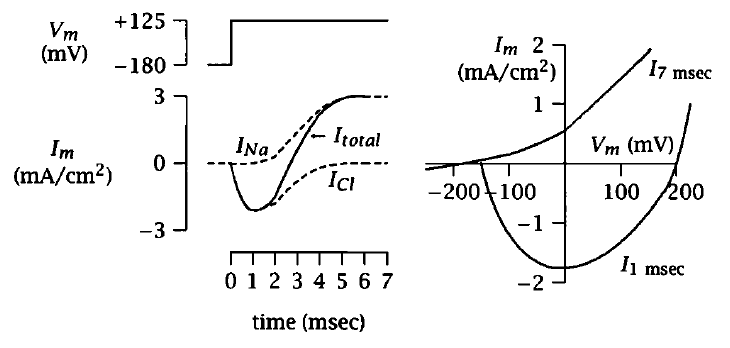
\includegraphics[width=0.75\textwidth]{/Users/jonathansun5/Documents/Fall 2017/MCB 166/Homeworks/HW 4/Screen Shot 2017-10-29 at 5.24.09 PM.png}
\end{center}
What are the values of $g_{\ch{Cl}}$ and $g_{\ch{Na}}$ at $Vm = -50 mV$ and at $Vm = +150 mV$?


\end{enumerate}



\newpage
\item
Which of the Hodgkin-Huxley variables, $m$, $h$, or $n$ is primarily responsible for each of the following phenomena: Explain your choice in one short sentence.
\begin{enumerate}[label=(\alph*)]
\item
Sharp threshold for excitation (for short-duration stimuli).



\item
Rapid repolarization at the end of an action potential.



\item
Undershoot after an action potential, ie. voltage is temporarily hyperpolarized beyond rest.



\item
Anode-break excitation, ie. membrane has lowered threshold after hyperpolarizing prepulse.



\end{enumerate}



\newpage
\item
The electric organ of the electric eel can generate a $600$ volt discharge. It is made up of stacks of about $4000$ asymmetric disc-shaped cells called electroplaques. The entire stack is surrounded by an insulating sheath, as shown in Fig. $1$. Each electroplaque has two different faces --- A and B in the figure. At rest, both faces are permeable to \ch{K+} and have relatively high resistance. At the peak of the action potential, face A has many activated \ch{Na+} channels, and thus has a low resistance and is permeable to \ch{Na+}. Face B is transiently activated by postsynaptic (acetylcholine) channels to trigger the action potential in face A. The acetylcholine channel is equally permeable to \ch{Na+} and \ch{K+} and has a reversal potential near zero. During activity this face also shows a low resistance.
\begin{center}
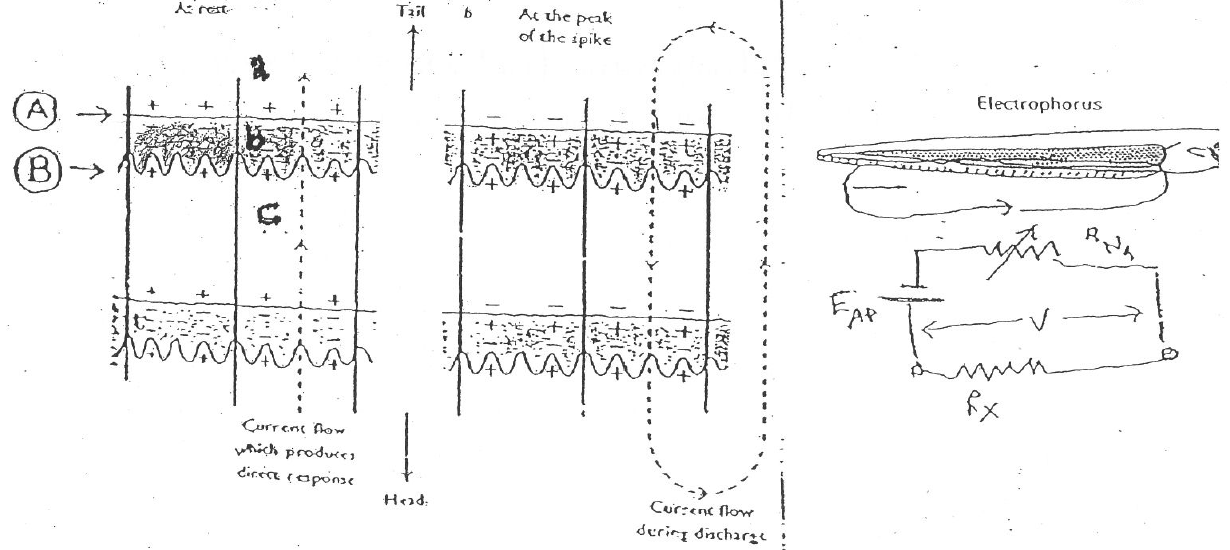
\includegraphics[width=0.75\textwidth]{/Users/jonathansun5/Documents/Fall 2017/MCB 166/Homeworks/HW 4/Screen Shot 2017-10-29 at 5.46.54 PM.png}
\end{center}
\begin{enumerate}[label=(\alph*)]
\item
Draw an equivalent circuit for the cell at rest and at peak activity representing the two membranes in series and using $V_{\ch{Na}} = +50 mV$ (inside relative to outside) and $V_{\text{rest}} = -90 mV$ (inside relative to outside). Calculate the resting potential and the action potential peak amplitude measured between microelectrodes placed at points a and b, and then between electrodes placed at a and c. $[\text{amplitude of AP} = V_{\text{AP}} - V_{\text{rest}}]$.







\item
Using the circuit diagram for a single electric cell, draw and label the equivalent circuit for the entire stack of $4000$ cells. Calculate the voltage drop across the stack at rest and at the action potential peak. Explain why the electric organ can generate such high voltages (sufficient to light up neon lights in aquariums). Why is it unlikely that a single excitable cell can be designed to generate voltages much higher than a few hundred millivolts?








\item
Complete the equivalent circuit for an electric organ composed of $4000$ electroplaques at peak discharge by sending surrent through an external resistance, $R_x$, the resistance of the medium through which the fish swims. Write an expression for the voltage the electric fish can utilize to stun its prey. There are both marine and fresh-water electric fish. Explain why the fresh-water types are more effective at stunning their prey. In fact, marine electric fish have only the excitable synaptic face with no electrically excitable face.







\item




\end{enumerate}

\newpage
\item
When a normal, healthy squid axon is voltage-clamped in artificial
sea water, one obtains the following membrane current record in response
to a step change in membrane potential from $V_m = -70 mV$
to $Vm = 0 mV$.
\begin{center}
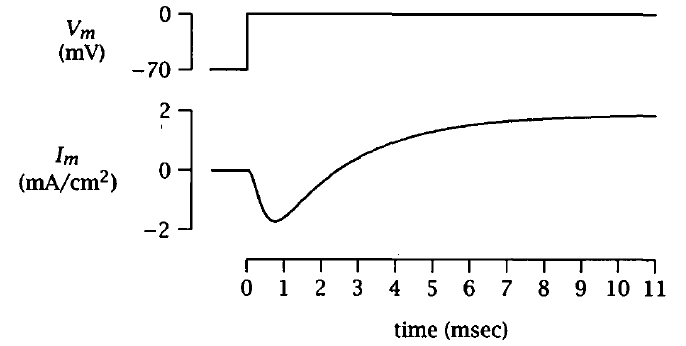
\includegraphics[width=0.75\textwidth]{/Users/jonathansun5/Documents/Fall 2017/MCB 166/Homeworks/HW 4/Screen Shot 2017-10-30 at 3.38.00 AM.png}
\end{center}
Draw similar plots of $I_m$ vs. $t$ (when $V_m$ is stepped from $- 70 mV$ to $0 mV$) when the recordings are made under each of the following experimental conditions. For each of your plots, explain in one or two sentences how and why your graph differs from that drawn above.
\begin{enumerate}[label=(\alph*)]
\item




\item




\item




\item




\item





\end{enumerate}









\end{enumerate}
\end{document}
